\documentclass{article}

% if you need to pass options to natbib, use, e.g.:
%     \PassOptionsToPackage{numbers, compress}{natbib}
% before loading neurips_2025

% The authors should use one of these tracks.
% Before accepting by the NeurIPS conference, select one of the options below.
\usepackage[main, final]{neurips_2025}

\usepackage[utf8]{inputenc} % allow utf-8 input
\usepackage[T1]{fontenc}    % use 8-bit T1 fonts
\usepackage{hyperref}       % hyperlinks
\usepackage{url}            % simple URL typesetting
\usepackage{booktabs}       % professional-quality tables
\usepackage{amsfonts}       % blackboard math symbols
\usepackage{nicefrac}       % compact symbols for 1/2, etc.
\usepackage{microtype}      % microtypography
\usepackage{xcolor}         % colors
\usepackage{amsmath}        % for math
\usepackage{graphicx}       % for graphics

\title{Individual Identification \\ on the Czech Lynx Dataset}

% The \author macro works with any number of authors.
\author{%
  
  Imad Elmakaoui\\
  Uniwersytet Jagielloński\\
  \texttt{imad.elmakaoui@student.uj.edu.pl} \\
  
}

\begin{document}

\maketitle

\begin{abstract}
Individual identification in wildlife monitoring is a challenging retrieval problem, particularly in unconstrained camera-trap environments. We propose an efficient individual identification framework utilizing Vision Transformers (ViTs) with an Efficient Probing mechanism for feature aggregation. By leveraging a pretrained DINOv3 backbone and learnable query-based aggregation, our method extracts discriminative features while maintaining computational efficiency through backbone feature caching. Evaluated on the Czech Lynx dataset, our approach achieves \textbf{33.0\% Top-1 accuracy}, significantly outperforming the standard MegaDescriptor baseline (19.0\%) and the specialized \textbf{Lynx-MegaDescriptor} (27.5\%). This represents a substantial improvement over existing methods, demonstrating the effectiveness of efficient token aggregation for fine-grained wildlife identification.
\end{abstract}

\section{Introduction}

Individual identification from images is an important task in wildlife monitoring and ecological research, as it enables non-invasive tracking of animals over time. The increasing use of camera traps has led to large collections of images captured under uncontrolled conditions, making manual identification impractical and motivating the development of automated methods.

This task is particularly challenging due to strong variations in illumination, viewpoint, background, and partial occlusions. In addition, individuals of the same species often exhibit only subtle visual differences, which limits the effectiveness of traditional feature-based approaches. As a result, robust identification systems must rely on learned visual representations that can generalize across diverse acquisition conditions.

Recent advances in deep learning have made it possible to learn such representations directly from data, allowing images to be compared based on similarity rather than fixed class assignments. However, applying large vision models in practice raises concerns related to computational efficiency and scalability, especially when high-resolution images are involved.

This project examines an efficient individual identification approach in a real-world wildlife monitoring setting, focusing on the use of pretrained vision models and similarity-based evaluation on the Czech Lynx dataset.

\begin{figure}[htbp]
\centering
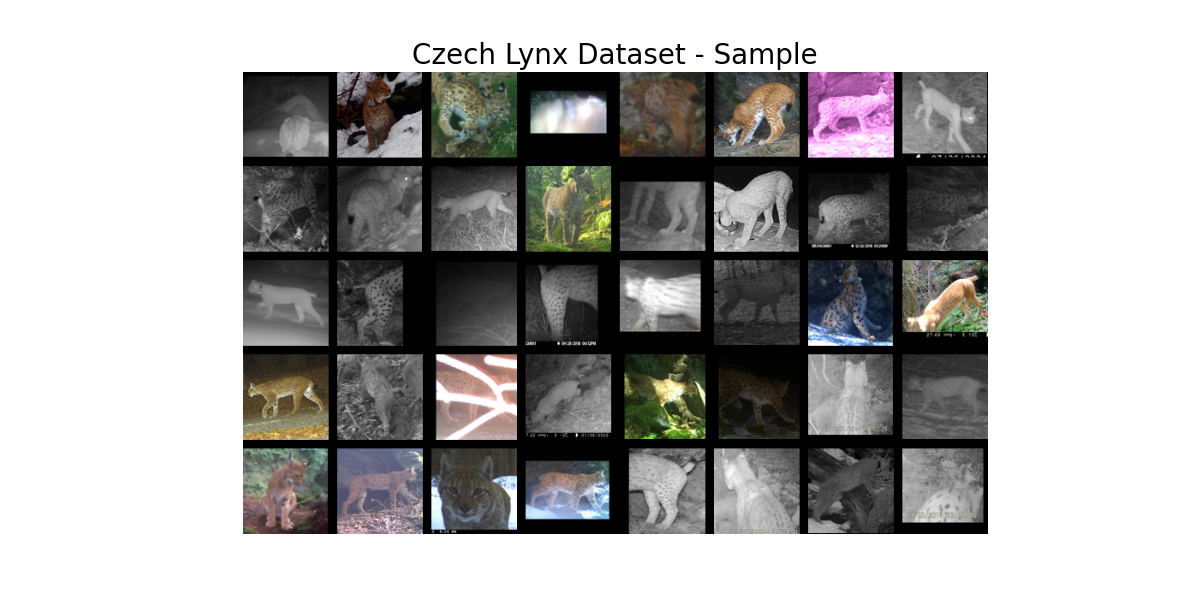
\includegraphics[width=1\linewidth]{Figure_1.png}
\caption{\label{fig:sample}Czech Lynx Dataset Sample.}
\end{figure}

\section{Related work}

\subsection{Handcrafted Feature-Based Approaches}

Early approaches to individual identification relied on handcrafted visual features and similarity measures designed to capture distinctive patterns such as color, texture, or shape. While these methods achieved moderate success in controlled settings, they often struggled in real-world scenarios due to sensitivity to illumination changes, viewpoint variations, and background clutter. This limitation is particularly evident in wildlife monitoring applications, where image acquisition conditions are largely uncontrolled.

\subsection{Deep Learning and Convolutional Neural Networks}

With the rise of deep learning, convolutional neural networks (CNNs) became the dominant approach for learning discriminative visual representations. CNN-based methods significantly improved performance by learning features directly from data and have been widely applied to re-identification tasks in both human and animal domains. However, CNNs primarily rely on local receptive fields, which can limit their ability to capture long-range dependencies and global contextual information, especially in images with complex backgrounds.

\subsection{Metric Learning for Individual Identification}

Metric learning has emerged as a key paradigm for individual identification. Instead of treating the task as a standard classification problem, metric learning methods aim to embed images into a feature space where samples of the same individual are close together and samples of different individuals are far apart. Loss functions such as triplet loss and contrastive loss are commonly used to enforce this structure and have shown strong performance in retrieval-based identification settings. These approaches are particularly suitable when the number of identities is large or when new identities may appear over time.

\subsection{Vision Transformers for Visual Representation Learning}

More recently, Vision Transformers (ViTs) have gained attention for visual representation learning due to their ability to model global relationships through self-attention mechanisms. By operating on patch-level tokens, ViTs can capture long-range dependencies that are difficult to model with convolutional architectures. Transformer-based models pretrained using self-supervised learning objectives have demonstrated strong generalization across a wide range of tasks, including image retrieval and re-identification.

\subsection{Efficient Adaptation of Pretrained Models}

Despite their effectiveness, transformer-based models are often computationally expensive to fine-tune, especially on high-resolution images. This has motivated research into efficient adaptation and aggregation strategies that can leverage pretrained representations while reducing computational cost. Lightweight token aggregation mechanisms and feature reuse strategies have been proposed to address these challenges.

\subsection{Summary and Motivation}
While deep learning has significantly advanced animal re-identification, current state-of-the-art methods often face a steep trade-off between computational cost and accuracy. Traditional CNN-based approaches and fully fine-tuned Vision Transformers require massive computational resources, which is often impractical for large-scale ecological monitoring projects involving tens of thousands of images. Our preliminary analysis of the Czech Lynx dataset—which contains nearly 40,000 images—revealed that while foundation models provide a strong latent-space starting point, they are not specifically optimized for the subtle intra-species variations of lynx in unconstrained environments.

The primary motivation for this work is to develop a framework that is both highly accurate and computationally scalable. By utilizing a DINOv3 backbone in conjunction with an Efficient Probing mechanism, we aim to leverage the global contextual power of Transformers while maintaining the parameter efficiency required for real-world deployment. Furthermore, the challenges discovered during our initial experiments—such as the instability of triplet loss on noisy camera-trap data and the detrimental effect of background clutter—motivated our investigation into variance-preserving noise infilling and robust contrastive objectives. Ultimately, this approach seeks to provide a scalable solution that can achieve significant performance gains, targeting the substantial relative improvements over baseline models required for reliable autonomous wildlife monitoring.

\section{Datasets}
\begin{figure}[htbp]
    \centering
    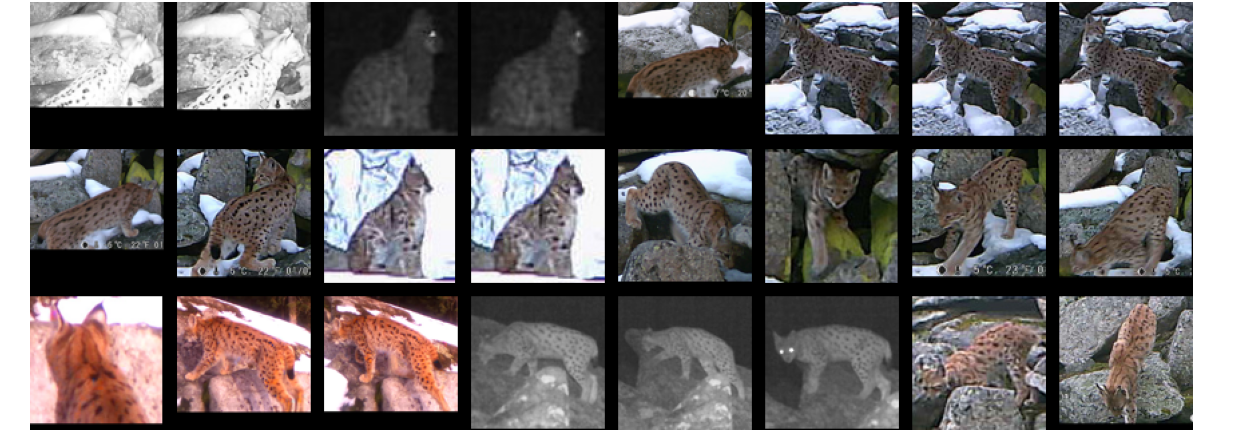
\includegraphics[width=\linewidth]{fig2.png}
    \caption{Czech Lynx Dataset Sample 2.}
    \label{fig:sample2}
\end{figure}

This work is conducted using the Czech Lynx dataset, a real-world wildlife dataset collected for the purpose of individual animal monitoring. The dataset consists of camera-trap images annotated with 319 individual identities, captured under unconstrained environmental conditions. As a result, the images exhibit significant variability in illumination, viewpoint, background, and image quality.

Geographically, the data is sourced from regions across Czechia, including the Bohemian and Carpathian mountain ranges. The dataset captures a wide range of environmental conditions across different monitoring stations (such as SNPA and FOE). This diversity introduces significant visual challenges, including varied illumination, complex forest backgrounds, and seasonal changes like snow-covered terrain, providing a rigorous benchmark for re-identification models.
Each image is associated with metadata describing the corresponding individual identity and acquisition context. To support individual identification, the dataset is divided ensuring that images of the same individual may appear in both training and evaluation sets, enabling retrieval-based evaluation. The dataset is split into training and test subsets, where the training set is used to learn feature representations and the test set is used for query-based identification.

During preprocessing, images are resized to a fixed resolution and standard normalization is applied. For part of the experiments, segmentation masks are used to reduce background influence by isolating the animal from its surroundings. This dataset provides a challenging and realistic benchmark for evaluating individual identification methods in wildlife monitoring scenarios.

\subsection{Statistical Background Infilling}

To mitigate the impact of complex forest backgrounds, we implemented a masking strategy using expert-provided segmentation masks. A critical finding in our preprocessing pipeline was that simple black-filling of the background introduced artificial sharp edges that negatively impacted model generalization. 

To address this, we utilized a variance-preserving noise strategy. For the masked background regions, we sampled noise from a normal distribution $N(\mu, \sigma^2)$, where the mean ($\mu$) and standard deviation ($\sigma$) were derived from global ImageNet statistics used during backbone pretraining. This approach maintains the statistical properties of the input data, preventing the model from over-fitting to the artificial boundaries of the mask and forcing it to focus exclusively on the discriminative features of the animal itself.

\section{Methodology}

\subsection{Problem Formulation}
The individual identification task is formulated as a retrieval problem rather than a traditional classification problem. Given an input image, the goal is to compute a feature embedding such that images of the same individual are mapped close to each other in the embedding space, while images of different individuals are mapped farther apart. Identification is performed by comparing embeddings using a distance metric and retrieving the most similar images from a reference database. In this work, Euclidean distance is used to measure similarity between image embeddings.

\subsection{Overall System Pipeline}
The proposed system follows a retrieval-based identification pipeline. Each input image is first preprocessed through resizing and normalization, and optionally through masking to reduce background influence. The preprocessed image is then passed through a pretrained vision model to extract patch-level visual features. These features are aggregated into a single compact embedding representing the image. During inference, embeddings of query images are compared against embeddings from a database to identify the most similar individuals.

\subsection{Efficient Probing and Backbone Selection}
Fine-tuning large-scale foundation models is often computationally prohibitive. To address this, we explored Efficient Probing \cite{psomas2025efficientprobing}, which utilizes attentive probing to optimize the trade-off between parameter efficiency and accuracy. While linear probing is a common baseline, attentive probing allows the model to selectively focus on discriminative visual tokens. 

We specifically investigated training an efficient probing head on top of DINOv3 \cite{Simeoni2025DINOv3} for Lynx re-identification. Previous literature has analyzed the latent-space separability of different species. This analysis confirmed that while these foundation models are not specifically trained on lynx, they provide a robust starting point for individual-level feature extraction \cite{Cermak_2024_WACV}. 

\subsection{Feature Extraction Backbone}
Feature extraction is performed using pretrained Vision Transformer models, which operate on image patches rather than individual pixels. The backbone produces a set of patch-level feature representations that capture both local visual patterns and global contextual information. Using pretrained models allows the system to leverage rich visual representations learned from large-scale datasets, improving generalization in scenarios with limited labeled data. In this work, different pretrained models are considered as feature extractors: DINOv3, MegaDescriptor, and LynxV4-MegaDescriptor-v2-T-256 \cite{lynx_megadescriptor} - a MegaDescriptor variant provided by one of the authors of the Czech Lynx dataset and fine-tuned for the Czech Lynx domain.

\subsection{Efficient Feature Aggregation}
The patch-level features produced by the backbone must be aggregated into a single representation suitable for retrieval. To achieve this, an efficient aggregation mechanism based on learnable queries is employed. These queries attend to the most informative regions of the image and selectively combine patch-level features into a compact embedding. This attention-based aggregation enables the model to focus on discriminative visual cues while reducing the dimensionality of the representation.

\subsection{Data Augmentation}
To simulate the challenging conditions of camera trap imagery and improve model robustness, we implemented a comprehensive augmentation pipeline. Beyond standard geometric transformations (random affine with rotation $\pm 15^\circ$, translation, scaling) and color jittering, we incorporated domain-specific augmentations designed to mimic environmental degradations:
\begin{itemize}
    \item \textbf{Blur effects}: Motion blur and defocus blur were applied to simulate animal movement and camera focus issues.
    \item \textbf{Atmospheric effects}: Synthetic fog and haze were generated to simulate weather conditions.
    \item \textbf{Noise and Exposure}: Gaussian noise, vignetting, and gamma correction were used to simulate sensor limitations and lighting variations.
    \item \textbf{Enhancement}: CLAHE (Contrast Limited Adaptive Histogram Equalization) and unsharp masking were applied to enhance local contrast and edge details, aiding in the discrimination of fine fur patterns.
\end{itemize}
We experimented with ablating the effect of different augmentations but did so with little success; we therefore settled on a smaller set of common-sense augmentations that slightly improved accuracy.

\subsection{Metric Learning with Structured PK-Sampling}
To optimize the embedding space, the model is trained using a \textbf{Contrastive Loss} (InfoNCE) with a temperature parameter of $\tau=0.07$. Effective training on this objective requires highly structured batches; we implemented a custom \textbf{PKSampler} to ensure that each batch contains $P$ unique individuals, with $K$ distinct images per individual. 

This structured batching provides the necessary positive and negative pairs for the model to learn to minimize intra-class variance while maximizing inter-class distance. We utilized an \textbf{AdamW} optimizer with a learning rate of $10^{-4}$ and a cosine annealing scheduler to maintain stability, particularly when training on the noisy camera-trap data where standard triplet mining proved difficult.

\subsection{Feature Space Visualization}
To gain qualitative insight into the learned representations, feature space visualizations are employed. By projecting high-dimensional embeddings into a two-dimensional space, it is possible to observe clustering patterns corresponding to individual identities. These visualizations provide an intuitive understanding of how different feature extractors structure the embedding space and complement quantitative evaluation metrics.

\begin{figure}[htbp]
    \centering
    \begin{minipage}{0.48\linewidth}
        \centering
        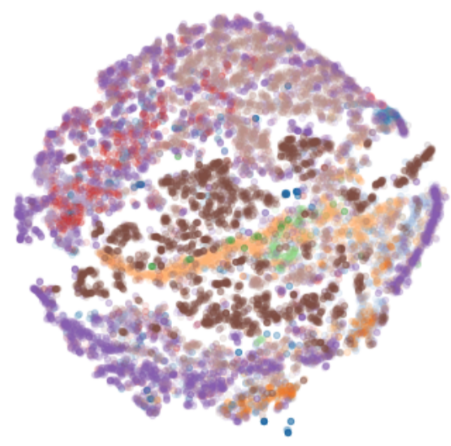
\includegraphics[width=\linewidth]{DINOV2.png}
        \caption{DINOv2 \cite{oquab2023dinov2} embedding visualization.}
        \label{fig:Dino}
    \end{minipage}
    \hfill
    \begin{minipage}{0.48\linewidth}
        \centering
        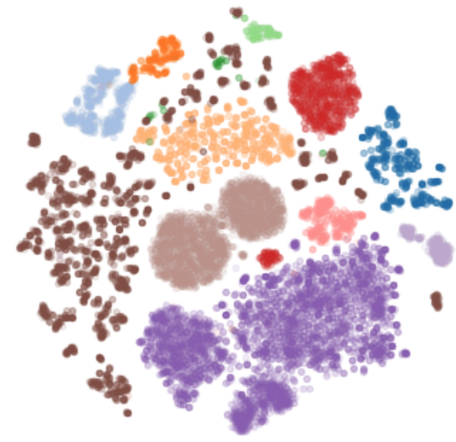
\includegraphics[width=\linewidth]{MegaDescriptor.png}
        \caption{MegaDescriptor-L-384 embedding visualization.}
        \label{fig:MDL384}
    \end{minipage}
\end{figure}

\section{Ablation Studies and Training Insights}
Our experimental process involved ablating several factors to determine the optimal configuration for camera-trap data:
\begin{itemize}
    \item \textbf{Background Infilling}: When using segmentation masks, we found that filling the background with variance-preserving noise significantly outperformed simple black filling. This prevents the model from over-relying on the sharp artificial edges created by the mask.
    \item \textbf{Loss Function Robustness}: Although triplet loss is a standard choice for metric learning, the inherent noise and high intra-class variance in the lynx dataset made triplet mining difficult. Contrastive loss proved to be more stable and effective in this specific domain.
    \item \textbf{Training Management}: We utilized the Weights \& Biases platform to track all training runs and model artifacts. This allowed us to monitor metrics like Top-1 accuracy across over a dozen configurations (such as "young-frog-121" and "silent-serenity-38"), ensuring reproducibility and enabling fast iteration.
\end{itemize}

\section{Implementation Details}

The proposed system is implemented using the \textbf{PyTorch} deep learning framework. All input images are resized to a fixed resolution of $384 \times 384$ pixels and normalized using standard \textbf{ImageNet statistics}. For experiments involving background suppression, segmentation masks are applied. We found that filling the background with \textbf{variance-preserving noise} yielded better results than black filling, as it prevents the model from latching onto artificial sharp edges created by the masking process.

We utilized \textbf{DINOv3 (ViT-Large)} as the feature extraction backbone. To ensure parameter efficiency, we kept the backbone \textbf{completely frozen} and trained only the Efficient Probing head. To improve computational efficiency, a \textbf{feature caching strategy} was employed, where backbone features were extracted once and stored on disk.

Training was optimized using \textbf{AdamW} with a learning rate of $10^{-4}$ and weight decay of $10^{-4}$. We used a batch size of \textbf{128} and trained for \textbf{20 epochs} with a cosine annealing learning rate scheduler. To ensure reproducibility and track experimental configurations, we utilized \textbf{Weights \& Biases} for all training runs.

Model evaluation follows a \textbf{retrieval-based protocol}. For each query image, \textbf{Euclidean distance} is used to compute similarity scores against a database of reference embeddings. Performance is reported using \textbf{top-K retrieval accuracy}, and qualitative analysis is supported through visualization of \textbf{retrieval results} and \textbf{feature space projections}.

\section{Evaluation}
\subsection{Evaluation Protocol}
The proposed approach is evaluated using a retrieval-based identification protocol. The dataset is divided into a database set, containing reference images of known individuals, and a query set, containing images to be identified. For each query image, a feature embedding is computed and compared against all database embeddings using a distance metric. The identity of the query is considered correctly identified if at least one image of the same individual appears among the top retrieved results. This protocol reflects realistic identification scenarios where a query must be matched against a large set of previously observed individuals.

\subsection{Evaluation Metrics}
Performance is measured using \textbf{Top-K retrieval accuracy}, which reports the proportion of query images for which the correct identity appears among the top K most similar database images. In particular, \textbf{Top-1 accuracy} evaluates whether the closest retrieved image corresponds to the correct individual, while \textbf{Top-K accuracy} (e.g., Top-3 or Top-5) accounts for cases where multiple plausible matches may exist. These metrics are commonly used in individual identification and re-identification tasks, as they directly reflect retrieval performance rather than classification accuracy.

\subsection{Baselines and comparisons}
To assess the effectiveness of the proposed approach, comparisons are conducted using different pretrained feature extractors under the same evaluation protocol. In particular, embeddings produced by \textbf{DINOv3}, \textbf{MegaDescriptor}, and \textbf{LynxV4-MegaDescriptor-v2-T-256} are evaluated as baseline representations. All methods are compared using identical dataset splits and distance metrics to ensure a fair comparison. This setup allows the impact of different representation learning strategies on identification performance to be analyzed objectively.
\begin{figure}[htbp]
    \centering
    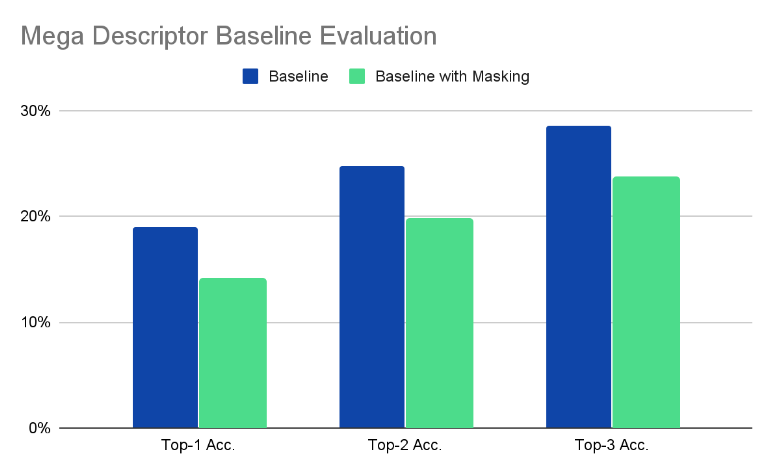
\includegraphics[width=0.6\linewidth]{Baselineeval.png}
    \caption{MegaDescriptor baseline evaluation.}
    \label{fig:baseline_eval}
\end{figure}

\section{Results}

The experimental results demonstrate the effectiveness of the proposed retrieval-based individual identification framework in a real-world wildlife monitoring scenario. Performance is evaluated using Top-K retrieval accuracy, which provides an objective measure of the system’s ability to correctly match query images with corresponding individuals in a reference database.

Table \ref{tab:results} presents the quantitative comparison between the baselines and our proposed method. The frozen MegaDescriptor-L-384 baseline achieves 19.0\% Top-1 accuracy. Interestingly, applying segmentation masks to the frozen baseline results in a performance drop to 14.1\% Top-1, suggesting that the background provides useful context for the pretrained model or that masking introduces artifacts. Our proposed approach (Fine-tuned + Efficient Probing) significantly outperforms both baselines, achieving \textbf{32.98\% Top-1 accuracy}, which corresponds to a relative improvement of approximately 70\% over the standard baseline.

\begin{table}[htbp]
    \centering
    \caption{Comparison of Top-K retrieval accuracy on the Czech Lynx dataset.}
    \label{tab:results}
    \begin{tabular}{lccc}
        \toprule
        \textbf{Method} & \textbf{Top-1} & \textbf{Top-2} & \textbf{Top-3} \\
        \midrule
        MegaDescriptor-L-384 (Baseline) & 19.0\% & 24.7\% & 28.6\% \\
        MegaDescriptor-L-384 (Masked) & 14.1\% & 19.7\% & 23.6\% \\
        MegaDescriptor-L-384 (Fine-tuned) & 24.1\% & 29.1\% & 32.7\% \\
        LynxV4-MegaDescriptor-v2-T-256 & 27.54\% & 33.22\% & 37.24\% \\
        DINOv3 & 23.02\% & 29.09\% & 33.10\% \\
        \textbf{Ours (DINOv3 + Efficient Probing)} & \textbf{32.98\%} & \textbf{40.17\%} & \textbf{44.36\%} \\
        \bottomrule
    \end{tabular}
\end{table}

Across all evaluated settings, fine-tuned representations consistently outperform baseline feature extractors, indicating improved discrimination between individuals in the learned embedding space. Quantitative improvements are supported by qualitative retrieval results, where the system successfully retrieves images of the same individual despite variations in viewpoint, illumination, and background conditions. In many cases, visually consistent matches are retrieved with high similarity scores, demonstrating robustness to common sources of visual variability in camera-trap imagery. Failure cases typically occur when individuals exhibit highly similar visual patterns or when images are captured under challenging conditions such as low illumination, occlusions, or motion blur.

Interestingly, DINOv3 alone achieves almost as good performance as the fine-tuned MegaDescriptor, indicating that it is quite capable of learning discriminative representations for individual identification. 

Overall, the results confirm that the proposed approach is capable of learning meaningful and discriminative representations for individual identification. While the system performs well under a variety of conditions, the remaining failure cases suggest that individual identification remains challenging in unconstrained environments, leaving room for future improvements through more robust feature aggregation or additional contextual information.

\begin{figure}[htbp]
    \centering
    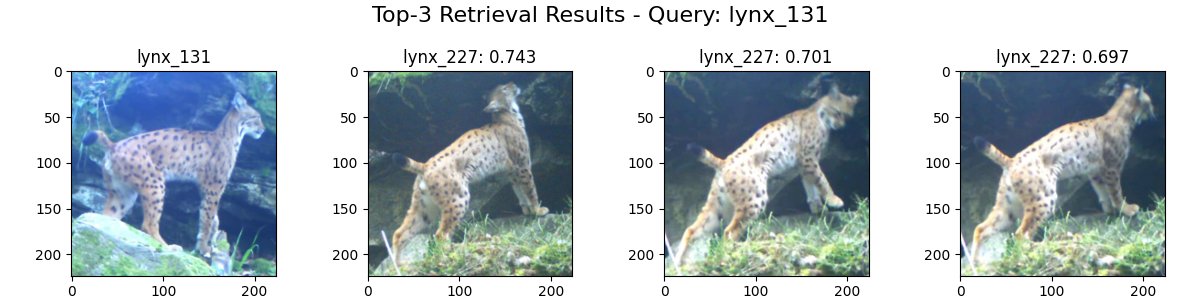
\includegraphics[width=0.45\linewidth]{top3.png}
    \hfill
    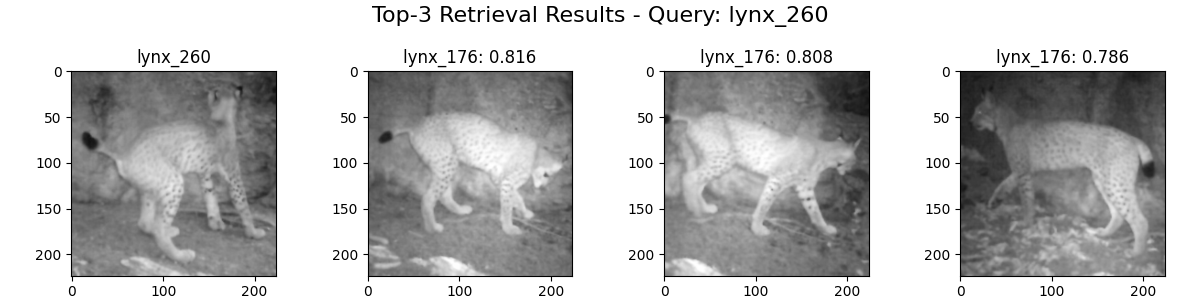
\includegraphics[width=0.45\linewidth]{top32.png}

    \vspace{0.5em}

    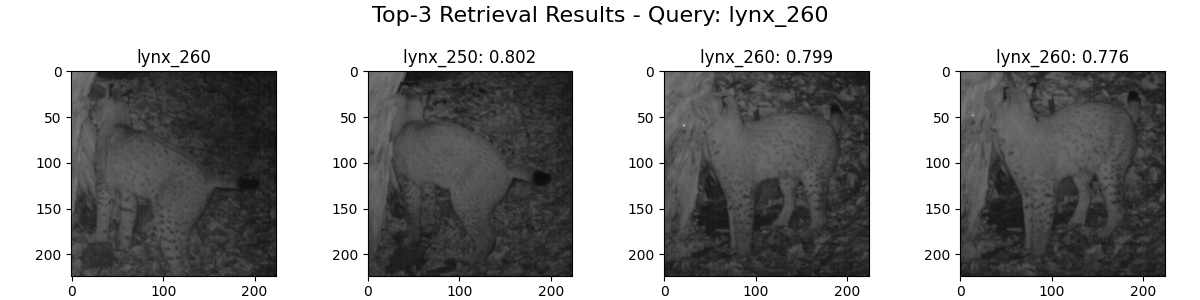
\includegraphics[width=0.45\linewidth]{top33.png}
    \hfill
    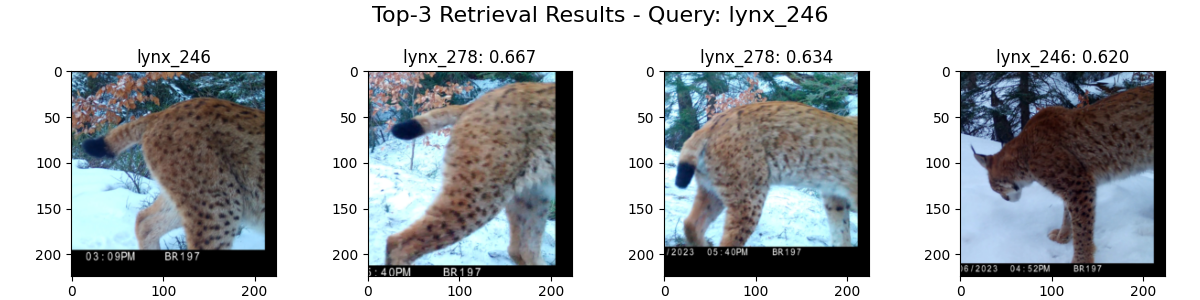
\includegraphics[width=0.45\linewidth]{top34.png}

    \caption{Retrieval results. }
    \label{fig:retrieval_results}
\end{figure}

\begin{figure}[htbp]
    \centering
    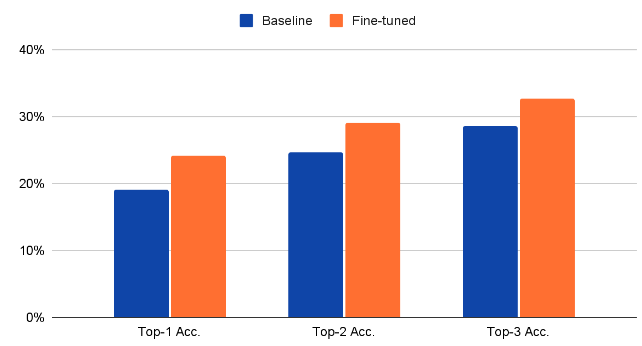
\includegraphics[width=0.6\linewidth]{MegaDescriptorfinetunedforczechlynx.png}
    \caption{MegaDescriptor fine-tuned for czech-lynx.}
    \label{fig:MGDF}
\end{figure}

\section{Conclusion and future work}
This work addressed the problem of individual identification in a wildlife monitoring context using a retrieval-based approach. By leveraging pretrained vision transformer models and metric learning objectives, the system learns discriminative feature embeddings that enable matching images of the same individual across challenging conditions. The proposed framework was evaluated on the Czech Lynx dataset using Top-K retrieval accuracy, qualitative retrieval examples, and feature space visualizations.

The experimental results demonstrate that fine-tuning pretrained representations, particularly the MegaDescriptor model, leads to consistent improvements in identification performance compared to baseline features. Quantitative gains in Top-K accuracy are supported by qualitative retrieval results and clearer clustering patterns in the embedding space, indicating improved separation between individuals. These findings confirm the effectiveness of adapting pretrained visual representations to domain-specific individual identification tasks.

Despite these encouraging results, individual identification in unconstrained environments remains challenging. Failure cases typically arise in situations involving poor image quality, strong occlusions, or visually similar individuals. Future work could explore more robust feature aggregation strategies, the incorporation of temporal information from camera-trap sequences, or the use of additional contextual cues to further improve identification performance. Evaluating generalization across multiple datasets and species also represents an important direction for extending this work.

\begin{ack}
I would like to thank my advisors, Adam Wróbel and Turhan Can Kargin, for their guidance and support throughout this project.
\end{ack}

The experiments in this work are conducted using the Czech Lynx dataset, a camera-trap dataset designed for individual animal identification under real-world conditions \cite{czechlynx}. 
Dataset preprocessing and management are supported by the WildlifeDatasets framework, which provides standardized tools for handling wildlife image datasets \cite{Cermak_2024_WACV}.

Feature extraction is performed using pretrained visual descriptors, including the MegaDescriptor-L-384 model, which provides compact and discriminative image representations suitable for retrieval-based identification \cite{megadescriptor}

The implementation relies on utilities provided by the WildlifeDatasets ecosystem, including tools for dataset handling, preprocessing, and experiment management \cite{wildlifetools}.

\bibliographystyle{plain}
\bibliography{references}
\end{document}
